\documentclass[12pt]{article}

\usepackage{booktabs}
\usepackage{dcolumn} 
\usepackage{epstopdf}
\usepackage{graphicx}
\usepackage{hyperref}
\usepackage{longtable} 
\usepackage{natbib}
\usepackage{rotating}
\usepackage{tabularx}
\usepackage{amsmath}
\usepackage{setspace}
\usepackage{caption}

%\usepackage[utf8]{inputenc}
%\usepackage[russian]{babel}


%\usepackage{fontawesome}
\usepackage[super]{nth}  
\hypersetup{
  colorlinks = TRUE,
  citecolor=blue,
  linkcolor=red,
  urlcolor=black
}

\hypersetup{colorlinks = TRUE, citecolor=blue, linkcolor=red, urlcolor=black}

\DeclareMathOperator*{\argmax}{arg\,max}

\newcommand{\starlanguage}{Significance indicators: $p \le 0.05:*$, $p \le 0.01:**$ and $p \le .001:***$.}

\newcommand{\covid}{Covid-19}  

\newtheorem{proposition}{Proposition}
\newtheorem{assumption}{Assumption}
\newtheorem{example}{Example}
\newtheorem{observation}{Observation}
\newtheorem{lemma}{Lemma}

\newcommand{\important}[1]{\textcolor{blue}{\textbf{ #1}}}
\newcommand{\quantclaim}[1]{\textcolor{red}{\textbf{ #1}}}


\newcommand{\LFPRhat}{58}
\newcommand{\numObs}{4,946}
\newcommand{\numObsWorking}{2,845}
\newcommand{\SurveyStart}{2020-06-29}
\newcommand{\SurveyEnd}{2020-07-04}
\newcommand{\LaidOff}{8.0}
\newcommand{\LaidOffLB}{4.5}
\newcommand{\LaidOffUB}{11.5}
\newcommand{\WFH}{28.4}
\newcommand{\WFHLB}{25.3}
\newcommand{\WFHUB}{31.5}
\newcommand{\alreadyWFH}{14.3}
\newcommand{\alreadyWFHLB}{10.9}
\newcommand{\alreadyWFHUB}{17.7}
\newcommand{\stillCommute}{42.7}
\newcommand{\stillCommuteLB}{40.0}
\newcommand{\stillCommuteUB}{45.5}


\begin{document} 

\title{Covid19 and Work-From-Home in the US:\\ An Early Look}

\date{\today}

\author{Erik Brynjolfsson\\Stanford \& NBER \and John Horton\\MIT \& NBER \and Adam Ozimek\\Upwork \and Daniel Rock\\MIT \and Garima Sharma\\MIT \and Hong Yi To Ye\\MIT}

\maketitle

\begin{abstract}
  \noindent The on-going \covid{} pandemic has confined large numbers of people to their homes and caused unprecedented lay-offs.
  In this note, we document TK. 
%  The timing of singups is consistent with 
  \newline 
%% \noindent JEL J01, J24, J3 \newline 
%% keywords: bargaining, match formation, wage determination
\end{abstract} 

\onehalfspacing 

\section{Introduction}
The on-going \covid{} pandemic has confined large numbers of people to their homes via quarntines and shelter-in-place orders.
Many businesses are closed. 
There have already been enormous and unprecendented increases in workers filing unemployment insurance claims \citep{goldsmith2020}. 

We conducted a survey on Google Consumer Surveys to get a sense of individual at-the-moment situation. 

We launched our survey on \SurveyStart{} and collected respondents until \SurveyEnd{}. 
We surveyed a total of \numObs{} respondents.
We asked a single question:
````Have you started to work from home in the last 4 weeks?''
which had the following response options: 

\begin{enumerate} 
\item ``I continue to commute to work''
\item ``I have recently been furloughed or laid-off''
\item ``None of the above / Not working for pay''
\item ``Used to commute, now work from home''   
\item ``Used to work from home and still do''       
\item ``Used to work from home, but now I commute''
\end{enumerate} 

\section{Results}

Of the respondents, \numObsWorking{} reported somethin other than ``None of the above / Not working for pay.''
This gives an implied labor force participation rate of \LFPRhat{}\%, which is lower than the BLS estimate about about 62\%, but still fairly close.
%Some of the ``None of above'' respondents could be unemployed. 
The distribution of answers pooled over all respondents is shown in Figure~\ref{fig:working_summary}. 

In Figure~\ref{fig:working_summary}, we can see that most common response was that they continue to commute, but the next most common was that they were now working from home. 
The working from home fraction is about 35\%. 
This is remarkably close to the estimate from \cite{dingel2020} that 34\% of jobs in the US can plausibly be performed from home.
As we will see, there is some regional variation, though we make no attempt to account for differing regions having different job compositions.

If we take the US labor force at about 165M, with an 11\% increase in furloughs/lay-offs, the impication is about ~16M recently out of work.
This is still considerably larger than the number who have reportedly filed for UI, as of April 1st, 2020.\footnote{
  \url{https://www.theguardian.com/business/2020/apr/02/us-unemployment-coronavirus-economy}
}

% 165 million
% https://fred.stlouisfed.org/series/CLF16OV

\begin{figure}
  \caption{Answers to the question ``Have you started to work from home in the last 4 weeks?'', conditional upon being in the labor force from a US sample} \label{fig:working_summary}
\centering
\begin{minipage}{1.0 \linewidth}
  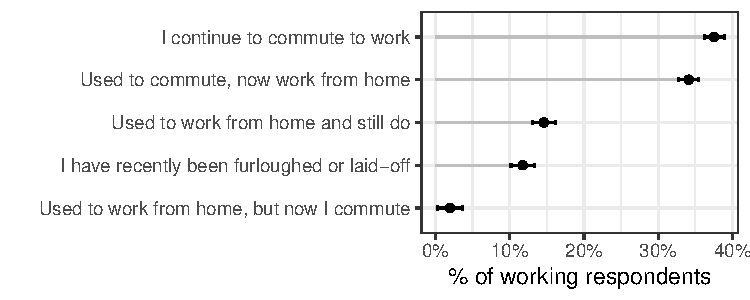
\includegraphics[width = \linewidth]{plots/working_summary.pdf} \\
  \begin{footnotesize}
    %% \begin{singlespace}
    %%   \emph{Notes:} 
    %% \end{singlespace}
    \end{footnotesize}
\end{minipage}
\end{figure} 

GCS also infers respondent gender.
We analyzed responses by gender but did not find any notable differences.
See Appendix~\ref{sec:gender}. 

\subsection{Geographic variation} 
Covid-19 has affected different parts of the US differently.
In Figure~\ref{fig:region}, we plot the fraction of respondents choosing each answer, by region.
GCS captures a respondents city and state, which are then mapped to the regions ``Northeast'', ``Midwest'', ``West'' and ``South.'' 

In the first facet from the left, we can see that the south has the highest fraction still commuting to work and the northeast has the lowest. 
In the second facet from the right, we can see that the northeast has the highest fraction of respondents switching to working from home, and the south the fewest.
The northeast started from the lowest fraction working from home, though these fractions are imprecisely estimated and are all fairly similar to each other. 
The northeast fraction now working from home is over 40\%, though the CI would just about reach the \cite{dingel2020} estimate.

\begin{figure}
  \caption{Responses by US region} \label{fig:region}
\centering
\begin{minipage}{1.0 \linewidth}
  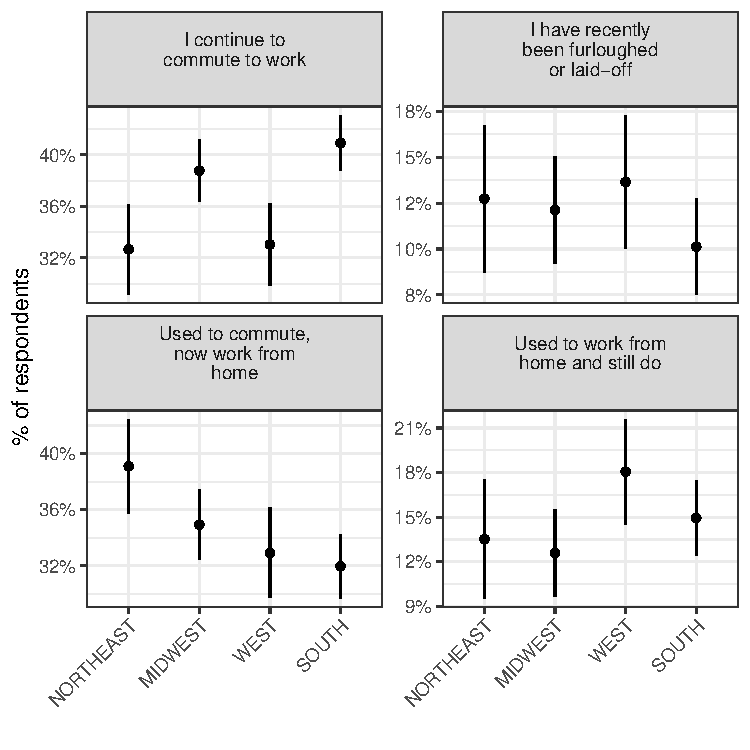
\includegraphics[width = \linewidth]{plots/region.pdf} \\
  \begin{footnotesize}
%    \begin{singlespace}
%      \emph{Notes:} Standard errors are reported. 
%    \end{singlespace}
    \end{footnotesize}
\end{minipage}
\end{figure} 

For a finer-grained look, we plot responses by state in Figure~\ref{fig:geo}. 
The fraction that are still continuing to commute to work is highest in the Dakatos, Wyoming and Montana.
The northeast, with the exception of Vermont shows large reductions in people still commuting to work. 

\begin{figure}
  \caption{Responses by US State} \label{fig:geo}
\centering
\begin{minipage}{1.0 \linewidth}
  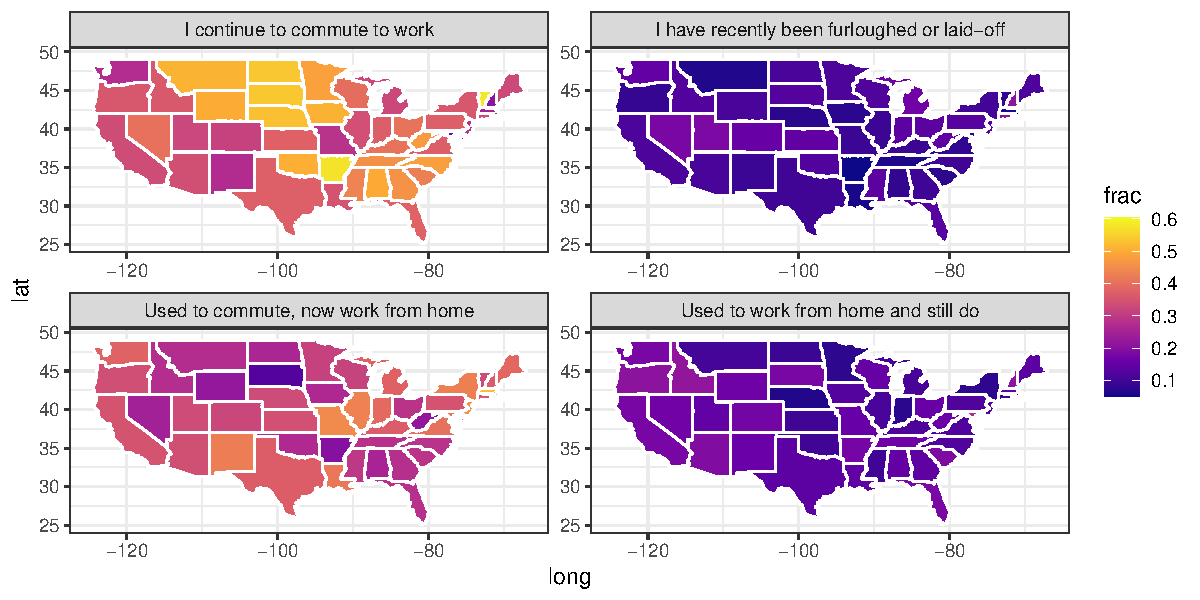
\includegraphics[width = \linewidth]{plots/geo.pdf} \\
  \begin{footnotesize}
    \begin{singlespace}
      \emph{Notes:} 
    \end{singlespace}
    \end{footnotesize}
\end{minipage}
\end{figure} 

\section{Conclusion}

\newpage \clearpage
\bibliographystyle{aer}
\bibliography{remote_work.bib}


\appendix

\section{Appendix} 
\subsection{By gender} \label{sec:gender}

In Figure~\ref{fig:gender} we report responses by inferred gender.

\begin{figure}
  \caption{Responses by gender} \label{fig:gender}
\centering
\begin{minipage}{1.0 \linewidth}
  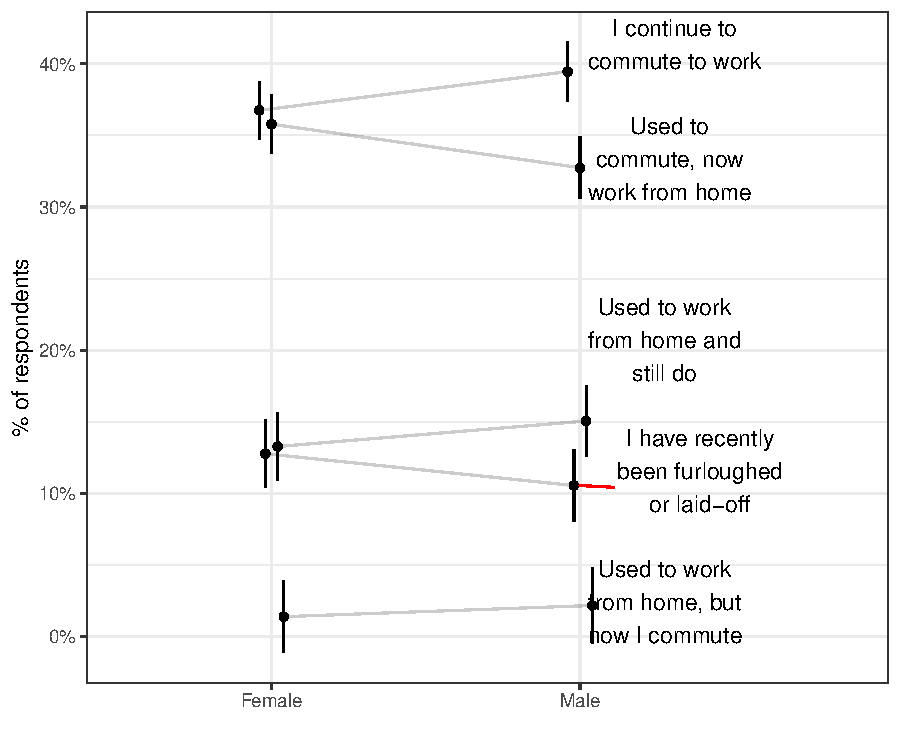
\includegraphics[width = \linewidth]{plots/gender.pdf} \\
  \begin{footnotesize}
    \begin{singlespace}
      \emph{Notes:} Standard errors are reported. 
    \end{singlespace}
    \end{footnotesize}
\end{minipage}
\end{figure} 

\end{document} 
